\documentclass[11pt]{article}

\usepackage{amsfonts}
\usepackage{amsmath, amsthm}
\usepackage{wasysym}
\usepackage{graphicx}
\usepackage{amssymb}
\usepackage{stmaryrd}
\usepackage{amsthm}
\usepackage{fancyhdr}
\usepackage[margin=1in]{geometry}
\usepackage[hang,flushmargin,symbol*]{footmisc}
\usepackage{color}
\definecolor{darkblue}{rgb}{0, 0, .6}
\definecolor{grey}{rgb}{.7, .7, .7}
\usepackage[breaklinks]{hyperref}
\hypersetup{
	colorlinks=true,
	linkcolor=darkblue,
	anchorcolor=darkblue,
	citecolor=darkblue,
	pagecolor=darkblue,
	urlcolor=darkblue,
	pdftitle={},
	pdfauthor={}
}

\newcommand{\dom}{\operatorname{Dom}}
\newcommand{\codom}{\operatorname{Codom}}
\newcommand{\range}{\operatorname{Rng}}

\pagestyle{fancy}

\lhead{\scriptsize Notes for an Introduction to Proof Course (Version Spring 2013)}
\rhead{\scriptsize Instructor: \href{http://danaernst.com}{D.C. Ernst}}
\lfoot{\scriptsize This work is an adaptation of notes written by Stan Yoshinobu of Cal Poly and Matthew Jones of California State University, Dominguez Hills.} 
\cfoot{}
\renewcommand{\headrulewidth}{0.4pt} 
\renewcommand{\footrulewidth}{0.4pt}


\theoremstyle{definition}
\newtheorem{theorem}{Theorem}[section]
\newtheorem{acknowledgement}[theorem]{Acknowledgement}
\newtheorem{algorithm}[theorem]{Algorithm}
\newtheorem{axiom}[theorem]{Axiom}
\newtheorem{case}[theorem]{Case}
\newtheorem{claim}[theorem]{Claim}
\newtheorem{conclusion}[theorem]{Conclusion}
\newtheorem{condition}[theorem]{Condition}
\newtheorem{conjecture}[theorem]{Conjecture}
\newtheorem{corollary}[theorem]{Corollary}
\newtheorem{criterion}[theorem]{Criterion}
\newtheorem{definition}[theorem]{Definition}
\newtheorem{example}[theorem]{Example}
\newtheorem{exercise}[theorem]{Exercise}
\newtheorem{journal}[theorem]{Journal}
\newtheorem{lemma}[theorem]{Lemma}
\newtheorem{notation}[theorem]{Notation}
\newtheorem{problem}[theorem]{Problem}
\newtheorem{proposition}[theorem]{Proposition}
\newtheorem{remark}[theorem]{Remark}
\newtheorem{solution}[theorem]{Solution}
\newtheorem{summary}[theorem]{Summary}
\newtheorem{question}[theorem]{Question}
\newtheorem{skeleton}[theorem]{Skeleton Proof}

\newsavebox{\savepar}
\newenvironment{textbox}{\noindent\begin{lrbox}{\savepar}\begin{minipage}[c]{.98\textwidth}}{\end{minipage}\end{lrbox}\fcolorbox{black}{white}{\usebox{\savepar}}}

\begin{document}

\addtocounter{section}{3}

\begin{section}{Two Famous Theorems (continued)}

\addtocounter{subsection}{1}
\addtocounter{theorem}{10}

\begin{subsection}{The irrationality of $\sqrt{2}$}

In this section\footnote{This section is derived from work of \href{}{Dave Richeson} of Dickenson College.} we will prove one of the oldest and most important theorems in mathematics. The Pythagoreans were an ancient secret society that followed their spiritual leader: Pythagoras of Samos (c.\ 570-495 BCE). The Pythagoreans believed that the way to spiritual fulfillment and to an understanding of the universe was through the study of mathematics. They believed that all of mathematics, music, and astronomy could be described via whole numbers and their ratios. In modern mathematical terms they believed that all numbers are rational. Attributed to Pythagoras is the saying, ``Beatitude is the knowledge of the perfection of the numbers of the soul.'' And their motto was ``All is number.''

Thus they were stunned when one of their own---Hippasus of Metapontum (c.\ 5th century BCE)---discovered that the side and the diagonal of a square are incommensurable. That is, the ratio of the length of the diagonal to the length of the side is irrational\footnote{Recall that a number is \textbf{rational} if it can be written in the form $\frac{m}{n}$, where $m,n\in\mathbb{Z}$ and $n\neq 0$.  A number is \textbf{irrational} if it is not rational.}. Indeed, if the side of the square has length $a$, then the diagonal will have length $a\sqrt{2}$; the ratio is $\sqrt{2}$ (see Figure~\ref{fig:square}).  In today's language, Hipassus discovery is given by the following theorem.

\begin{figure}[ht]
\begin{center}
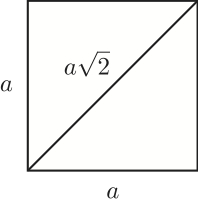
\includegraphics{square}
\end{center}
\vspace{-.5cm}
\caption{The side and diagonal of a square are incommensurable.}
\label{fig:square}
\end{figure}

\begin{theorem}[*]
\label{thm:sqrt2}
The real number $\sqrt{2}$ is irrational\footnote{\emph{Hint:} Use a proof by contradiction.  That is, suppose that there exist $m,n\in\mathbb{Z}$ such that $n\ne 0$ and $\sqrt{2}=\frac{m}{n}$. Moreover, assume $m$ and $n$ have no common factors.  Derive a contradiction using Theorem~???.}.
\end{theorem}

As one might expect, the Pythagoreans were unhappy with this discovery. Legend says that Hippasus was expelled from the Pythagoreans and was perhaps drowned at sea. Ironically, this result, which angered the Pythagoreans so much, is probably their greatest contribution to mathematics: the discovery of irrational numbers.

Now, let's tackle a few more problems dealing with irrational numbers.

\begin{problem}
Determine whether $\displaystyle \frac{1+\sqrt{2}}{3+2\sqrt{2}}$ is rational or irrational and then prove that your answer is correct.
\end{problem}

\begin{theorem}[*]
Let $p$ be a prime number.  Then $\sqrt{p}$ is irrational.
\end{theorem}

\begin{exercise}
Let $p$ be a prime number.  For which values of $n\in\mathbb{N}$ is $\sqrt[n]{p}$ irrational?  You do not need to prove your answer.
\end{exercise}

\begin{theorem}[*]\label{thm:sqrt(pq)}
Let $p$ and $q$ be distinct primes.  Then $\sqrt{pq}$ is irrational.
\end{theorem}

\begin{problem}
State a generalization of Theorem~\ref{thm:sqrt(pq)} and briefly describe how its proof would go.  Be as general as possible.
\end{problem}

\begin{remark}
It is important to point out that not every positive irrational number is equal to the square root of some natural number.  For example, $\pi$ is irrational, but is not equal to the square root of a natural number.
\end{remark}

\end{subsection}

\end{section}

\end{document}